\documentclass[12pt, a4paper]{article}

% --- Packages ---
\usepackage[utf8]{inputenc}
\usepackage[T1]{fontenc}
\usepackage[italian]{babel}
\usepackage{amsmath, amssymb}
\usepackage{graphicx}
\usepackage{booktabs}
\usepackage{hyperref}
\usepackage{natbib}
\usepackage{geometry}
\usepackage{caption}
\usepackage{subcaption}
\usepackage{float}
\usepackage{microtype}
\usepackage{setspace}
\usepackage{abstract}

\geometry{margin=2.5cm}
\onehalfspacing
\hypersetup{colorlinks=true, linkcolor=black, citecolor=black, urlcolor=blue}

% Etichetta italiana per l'abstract
\renewcommand{\abstractname}{Sommario}

% --- Metadata ---
\title{I Magnifici Sette e l'efficienza dei mercati:\\
scomporre i rendimenti dell'S\&P500 attraverso\\
l'analisi della concentrazione (2019--2024)}

\author{
  Giulio Parrinello\\
  \small Universit\`a degli Studi di Palermo\\
  \small  Corso di studi in Ingegneria Gestionale\\
  \small \texttt{giulioparrinello@mail.com}
}

\date{\today}

% --- Document ---
\begin{document}
\maketitle

\begin{abstract}
Questo articolo indaga in che misura la performance degli ultimi sei anni dell'indice S\&P500 (2019--2024) sia attribuibile a un ristretto sottoinsieme di grandi aziende tecnologiche, comunemente note come  ``Magnifici Sette'' (Apple, Microsoft, NVIDIA, Amazon, Alphabet, Meta e Tesla). Utilizzando dati di prezzo giornaliero pubblicamente disponibili, il numero \emph{storico} di azioni in circolazione per ricostruire pesi di capitalizzazione di mercato variabili nel tempo, e l'ETF equiponderato dell'S\&P500 (RSP) come benchmark neutrale rispetto alla concentrazione, scomponiamo i rendimenti dell'indice e quantifichiamo l'effetto-concentrazione. Troviamo che l'indice ponderato per capitalizzazione (SPY, $+158\%$) ha sovraperformato la propria versione equiponderata (RSP, $+113\%$) di circa $46$ punti percentuali; che i Magnifici Sette sono cresciuti da circa il $16\%$ al $58\%$ della capitalizzazione di mercato dei cinquanta maggiori titoli; e che un indice controfattuale che escludesse queste sette aziende avrebbe reso $+108\%$ invece di $+167\%$, il che implica che il gruppo spiega circa il $35\%$ dei rendimenti cumulati dell'indice. Questi risultati sollevano interrogativi sulle assunzioni di diversificazione insite nell'investimento passivo e sul contenuto empirico della forma semi-forte dell'Ipotesi dei Mercati Efficienti in un'epoca di concentrazione del capitale.
\end{abstract}

\section{Introduzione}

L'indice S\&P500 è ampiamente considerato un termometro diversificato del mercato azionario statunitense. Per costruzione, tuttavia, esso è \emph{ponderato per capitalizzazione}: ogni azienda entra nell'indice in proporzione al proprio valore di mercato, sicché le società più grandi esercitano un'influenza sproporzionata sul comportamento dell'indice. Negli ultimi anni questo meccanismo ha prodotto una concentrazione senza precedenti del peso dell'indice in un piccolo numero di mega-aziende a guida tecnologica --- Apple, Microsoft, NVIDIA, Alphabet, Amazon, Meta e Tesla --- collettivamente noti come i ``Magnifici Sette''.

Questo articolo pone una domanda semplice ma empiricamente importante: \emph{quanta parte della performance cumulata dell'S\&P500 nel periodo 2019--2024 è attribuibile a queste sette aziende, e che cosa ciò implica per l'efficienza del mercato?} Rispondiamo in tre modi complementari. In primo luogo, confrontiamo l'indice standard ponderato per capitalizzazione (rappresentato da SPY) con la versione equiponderata dello stesso indice (rappresentata dall'ETF RSP); il divario tra i due è la misura di mercato più pulita di quanto abbia contato la concentrazione. In secondo luogo, ricostruiamo pesi di capitalizzazione \emph{variabili nel tempo} a partire dai dati storici sulle azioni in circolazione e costruiamo un indice controfattuale che esclude i Magnifici Sette. In terzo luogo, scomponiamo i contributi al rendimento anno per anno e azienda per azienda. In tutto il lavoro mettiamo in relazione i risultati con l'Ipotesi dei Mercati Efficienti \citep{fama1970, fama1991}.

\section{Rassegna della letteratura}

\subsection{L'Ipotesi dei Mercati Efficienti}

\citet{fama1970} introdusse la classica tassonomia in tre forme dell'efficienza di mercato. La forma semi-forte postula che i prezzi riflettano pienamente tutte le informazioni pubblicamente disponibili, implicando che nessun investitore possa ottenere sistematicamente rendimenti anomali tramite l'analisi fondamentale. \citet{fama1991} ha in seguito raffinato il quadro teorico, riconoscendo il problema della doppia ipotesi che affligge tutti i test empirici dell'efficienza: ogni test dell'efficienza è simultaneamente un test del modello di pricing degli attivi che si è assunto.

\subsection{Le critiche della finanza comportamentale}

\citet{shiller1981} ha dimostrato che i prezzi azionari esibiscono una ``volatilità eccessiva'' rispetto alle successive variazioni dei dividendi, mettendo in discussione il fondamento di aspettative razionali dell'EMH. \citet{debondt1985} ha documentato una iper-reazione sistematica, con i titoli precedentemente perdenti che battono i precedenti vincitori su orizzonti di tre-cinque anni. Questi risultati suggeriscono che i mercati possano non incorporare le informazioni in modo efficiente a tutti gli orizzonti temporali, in particolare durante episodi di entusiasmo speculativo.

\subsection{La concentrazione mega-cap negli indici moderni}

Ricerche recenti e commenti di mercato \citep{sp500mag7_2024} hanno messo in evidenza la crescente concentrazione dell'S\&P500 attorno a una manciata di aziende tecnologiche. Il fenomeno è storicamente insolito: il peso combinato dei principali costituenti nel 2024 ha raggiunto livelli non più visti dagli anni '70, quando AT\&T e IBM dominavano l'indice. Le implicazioni per gli investitori passivi --- che per costruzione detengono l'indice così com'è --- sono significative, poiché la diversificazione che credono di possedere è sempre più nominale. Il caso classico a favore della diversificazione risale a \citet{markowitz1952}.

\section{Dati e metodologia}

\subsection{Fonti dei dati}

I prezzi di chiusura giornalieri provengono da Yahoo Finance tramite la libreria Python \texttt{yfinance}. Utilizziamo l'ETF SPY come proxy dell'S\&P500 ponderato per capitalizzazione e l'ETF Invesco RSP come proxy dell'S\&P500 equiponderato. Il periodo di analisi va dal 2 gennaio 2019 al 31 dicembre 2024 ($1{,}509$ giorni di contrattazione).

Un miglioramento metodologico chiave rispetto alle analisi statiche riguarda il nostro trattamento dei pesi. Anziché applicare retroattivamente i pesi di indice \emph{attuali} --- il che introdurrebbe un \emph{look-ahead bias} a favore delle aziende che sono grandi \emph{oggi} --- ricostruiamo le capitalizzazioni di mercato \emph{storiche} come prodotto tra il prezzo di chiusura non rettificato di ciascuna azienda e le sue azioni in circolazione a ciascuna data, queste ultime ottenute dalla serie storica delle azioni in circolazione di Yahoo Finance. Ne risultano pesi variabili nel tempo che riflettono la dimensione effettiva di ciascuna azienda in ciascun istante.

\subsection{Ricostruzione dell'indice}

Definiamo l'universo di lavoro come i cinquanta maggiori costituenti dell'S\&P500 per capitalizzazione di mercato media nel periodo, i quali insieme rappresentano la grande maggioranza del valore dell'indice e ne riproducono fedelmente l'andamento complessivo (il rendimento ponderato per capitalizzazione ricostruito è correlato a $\rho = 0{,}98$ con SPY, a conferma della validità dell'approccio). Per costruire l'indice controfattuale ``senza Magnifici Sette'' rimuoviamo i sette ticker esclusi e rinormalizziamo quotidianamente i pesi rimanenti. Formalmente, per i costituenti rimanenti $i \in I \setminus E$, dove $E$ è l'insieme degli esclusi:
\begin{equation}
  w_{i,t}^{*} = \frac{m_{i,t}}{\sum_{j \in I \setminus E} m_{j,t}}, \qquad
  m_{i,t} = p_{i,t}\, s_{i,t},
\end{equation}
dove $p_{i,t}$ è il prezzo non rettificato e $s_{i,t}$ le azioni in circolazione. Il rendimento giornaliero controfattuale è
\begin{equation}
  r_t^{\text{ex}} = \sum_{i \in I \setminus E} w_{i,t-1}^{*} \cdot r_{i,t}.
\end{equation}

\subsection{Performance corretta per il rischio}

Il confronto corretto per il rischio si basa sullo Sharpe ratio. Anziché fissare il tasso privo di rischio, utilizziamo il rendimento \emph{realizzato} dei Treasury bill statunitensi a 13 settimane (\texttt{\^{}IRX}), che è variato da quasi zero nel 2020--2021 a oltre il $5\%$ nel 2023--2024. Lo Sharpe ratio annualizzato è calcolato sia sull'intero periodo sia su una finestra mobile di 12 mesi (252 giorni):
\begin{equation}
  \mathrm{Sharpe} = \frac{\overline{r_t - r^{f}_t}}{\sigma(r_t - r^{f}_t)} \, \sqrt{252}.
\end{equation}

\subsection{Limiti}

\begin{itemize}
  \item L'universo di lavoro è costituito dai primi 50 costituenti; i membri più piccoli dell'S\&P500 sono esclusi, sebbene il loro peso aggregato sia ridotto.
  \item SPY e RSP sono usati come proxy dell'indice e della sua versione equiponderata; sussistono un modesto errore di replica e l'attrito dovuto alle commissioni.
  \item I dati sulle azioni in circolazione sono comunicati a intervalli irregolari e riportati in avanti (forward-fill) tra un aggiornamento e l'altro.
  \item La composizione stessa dei ``Magnifici Sette'' è scelta col senno di poi; il gruppo è definito ex post come l'insieme delle aziende che sono arrivate a dominare l'indice.
  \item Il periodo include eventi macroeconomici eccezionali (il crollo da Covid, il mercato rialzista post-Covid e lo shock dei tassi del 2022) che amplificano l'effetto-concentrazione misurato.
\end{itemize}

\section{Risultati}

\subsection{Confronto delle performance}

\begin{figure}[H]
  \centering
  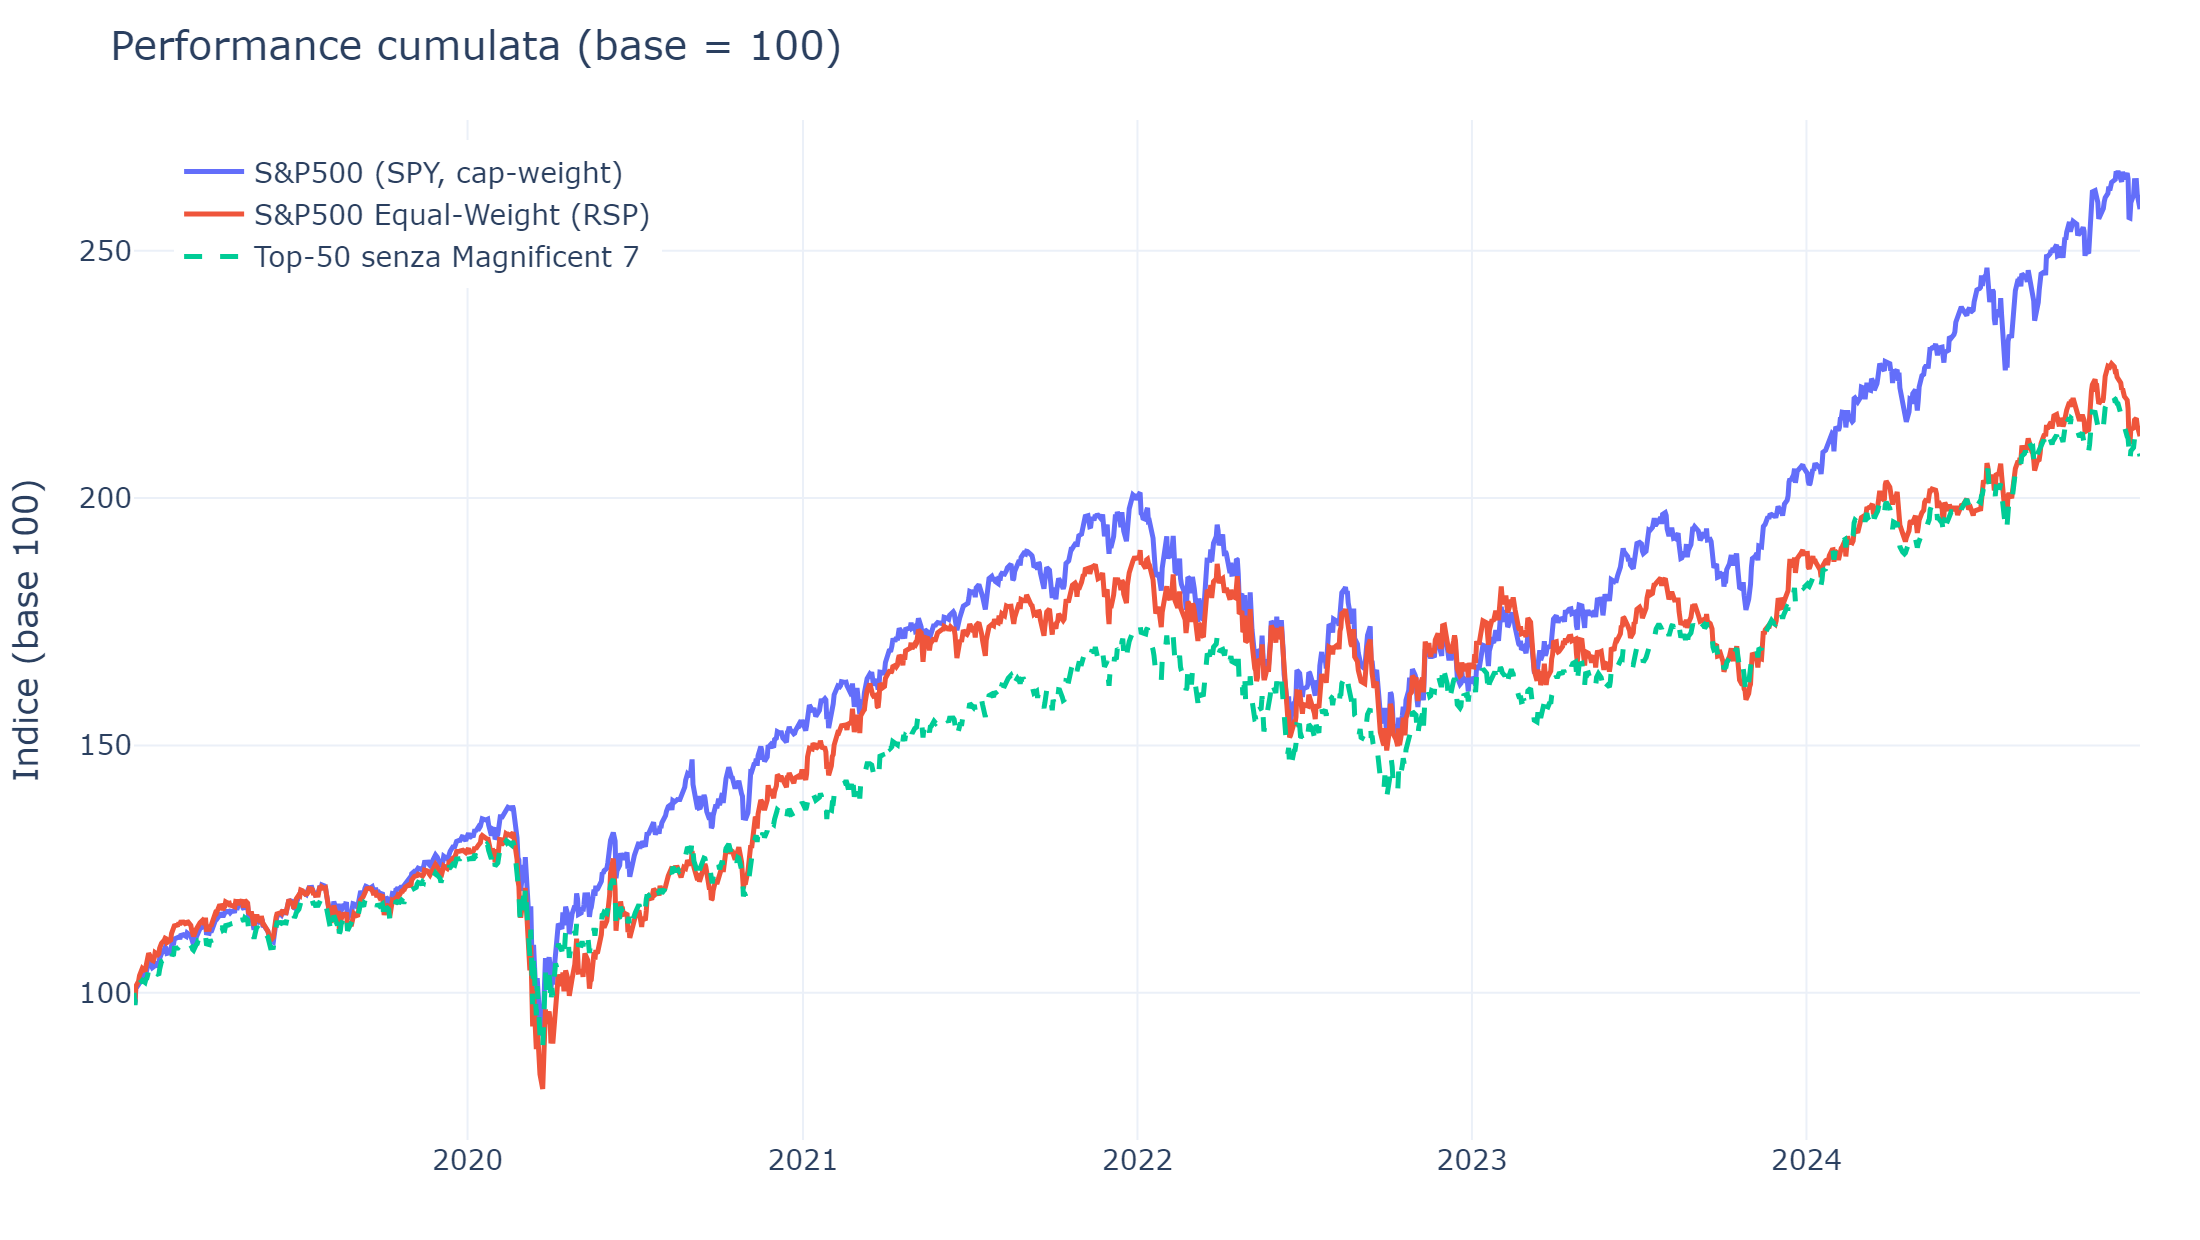
\includegraphics[width=\linewidth]{figures/performance_chart.png}
  \caption{Performance cumulata (base $=100$): l'S\&P500 ponderato per capitalizzazione (SPY), la sua versione equiponderata (RSP) e l'indice ricostruito dei primi 50 titoli escludendo i Magnifici Sette, 2019--2024.}
  \label{fig:performance}
\end{figure}

La Figura~\ref{fig:performance} mostra il risultato centrale. L'indice ponderato per capitalizzazione ha reso $+158\%$ nel periodo, mentre la versione equiponderata ha reso soltanto $+113\%$ --- un divario di circa $46$ punti percentuali attribuibile quasi interamente al contributo sproporzionato delle aziende più grandi. L'indice controfattuale dei primi 50 titoli che esclude i Magnifici Sette resta ancora più indietro, a $+108\%$. Le tre curve sono pressoché indistinguibili fino al 2020, per poi divaricarsi progressivamente, con la divergenza che accelera nettamente nel biennio 2023--2024.

\subsection{Attribuzione dei rendimenti}

\begin{figure}[H]
  \centering
  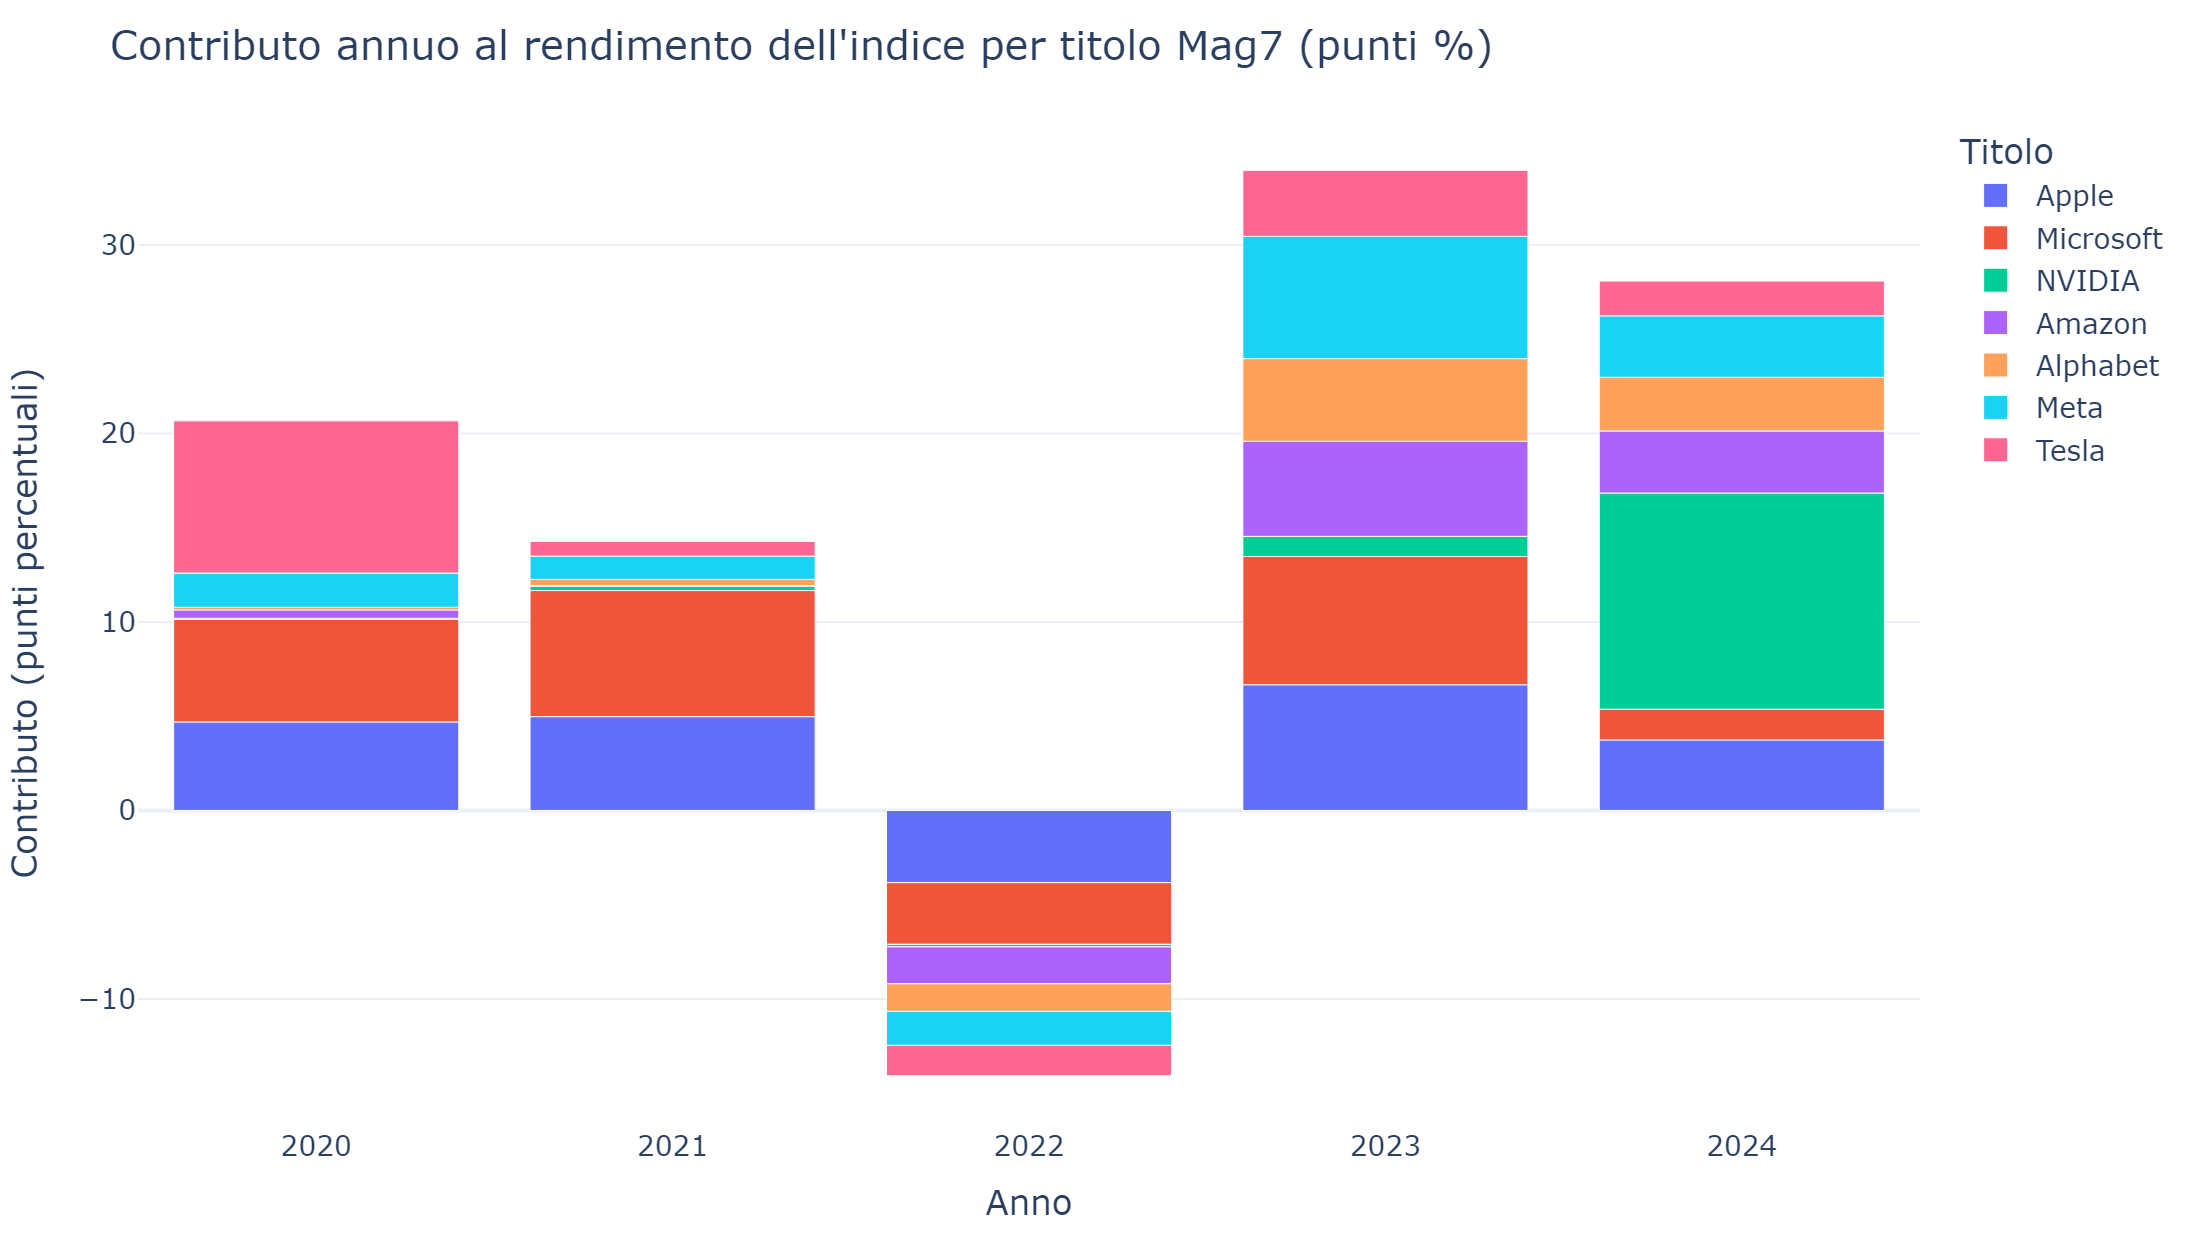
\includegraphics[width=\linewidth]{figures/attribution_chart.png}
  \caption{Contributo annuo al rendimento dell'indice per ciascun titolo dei Magnifici Sette (punti percentuali di rendimento dell'indice), utilizzando i pesi storici variabili nel tempo.}
  \label{fig:attribution}
\end{figure}

La scomposizione a livello di singola azienda (Figura~\ref{fig:attribution}) mostra che il contributo non è distribuito in modo uniforme. Nel solo biennio 2023--2024, NVIDIA ha aggiunto circa $12{,}5$ punti percentuali al rendimento dell'indice, Apple $10{,}4$, Meta $9{,}8$, Microsoft $8{,}4$, Amazon $8{,}3$, Alphabet $7{,}2$ e Tesla $5{,}4$. L'emergere di NVIDIA come singolo maggiore contributore nel 2023--2024, sulla scia del ciclo di investimenti nell'intelligenza artificiale, è la caratteristica più sorprendente del periodo.

\begin{table}[H]
  \centering
  \caption{Riepilogo delle metriche principali, 2019--2024. Gli Sharpe ratio utilizzano il tasso realizzato dei T-bill a 13 settimane.}
  \begin{tabular}{lrrrr}
    \toprule
    & SPY (cap-wt) & RSP (equipond.) & Senza Mag7 & Solo Mag7 \\
    \midrule
    Rendimento cumulato       & $158{,}4\%$ & $112{,}5\%$ & $108{,}5\%$ & $364{,}7\%$ \\
    Rendimento annualizzato   & $17{,}2\%$  & $13{,}4\%$  & $13{,}1\%$  & $29{,}2\%$ \\
    Volatilità annualizzata   & $19{,}8\%$  & $20{,}9\%$  & $18{,}2\%$  & $28{,}6\%$ \\
    Sharpe ratio              & $0{,}78$    & $0{,}59$    & $0{,}63$    & $0{,}96$ \\
    Max drawdown              & $-33{,}7\%$ & $-39{,}0\%$ & $-32{,}1\%$ & $-43{,}3\%$ \\
    \bottomrule
  \end{tabular}
  \label{tab:metrics}
\end{table}

La Tabella~\ref{tab:metrics} rivela un punto più sottile. I Magnifici Sette non si sono limitati ad alzare i rendimenti; su base autonoma hanno conseguito uno Sharpe ratio di $0{,}96$, ben superiore sia all'indice ponderato per capitalizzazione ($0{,}78$) sia a quello equiponderato ($0{,}59$), nonostante una volatilità assai più elevata ($28{,}6\%$) e un drawdown più profondo ($-43{,}3\%$). La superiorità dello Sharpe dell'indice ponderato per capitalizzazione rispetto alla versione equiponderata è dunque ereditata direttamente dalla sua concentrazione su questi nomi.

\subsection{La concentrazione nel tempo}

\begin{figure}[H]
  \centering
  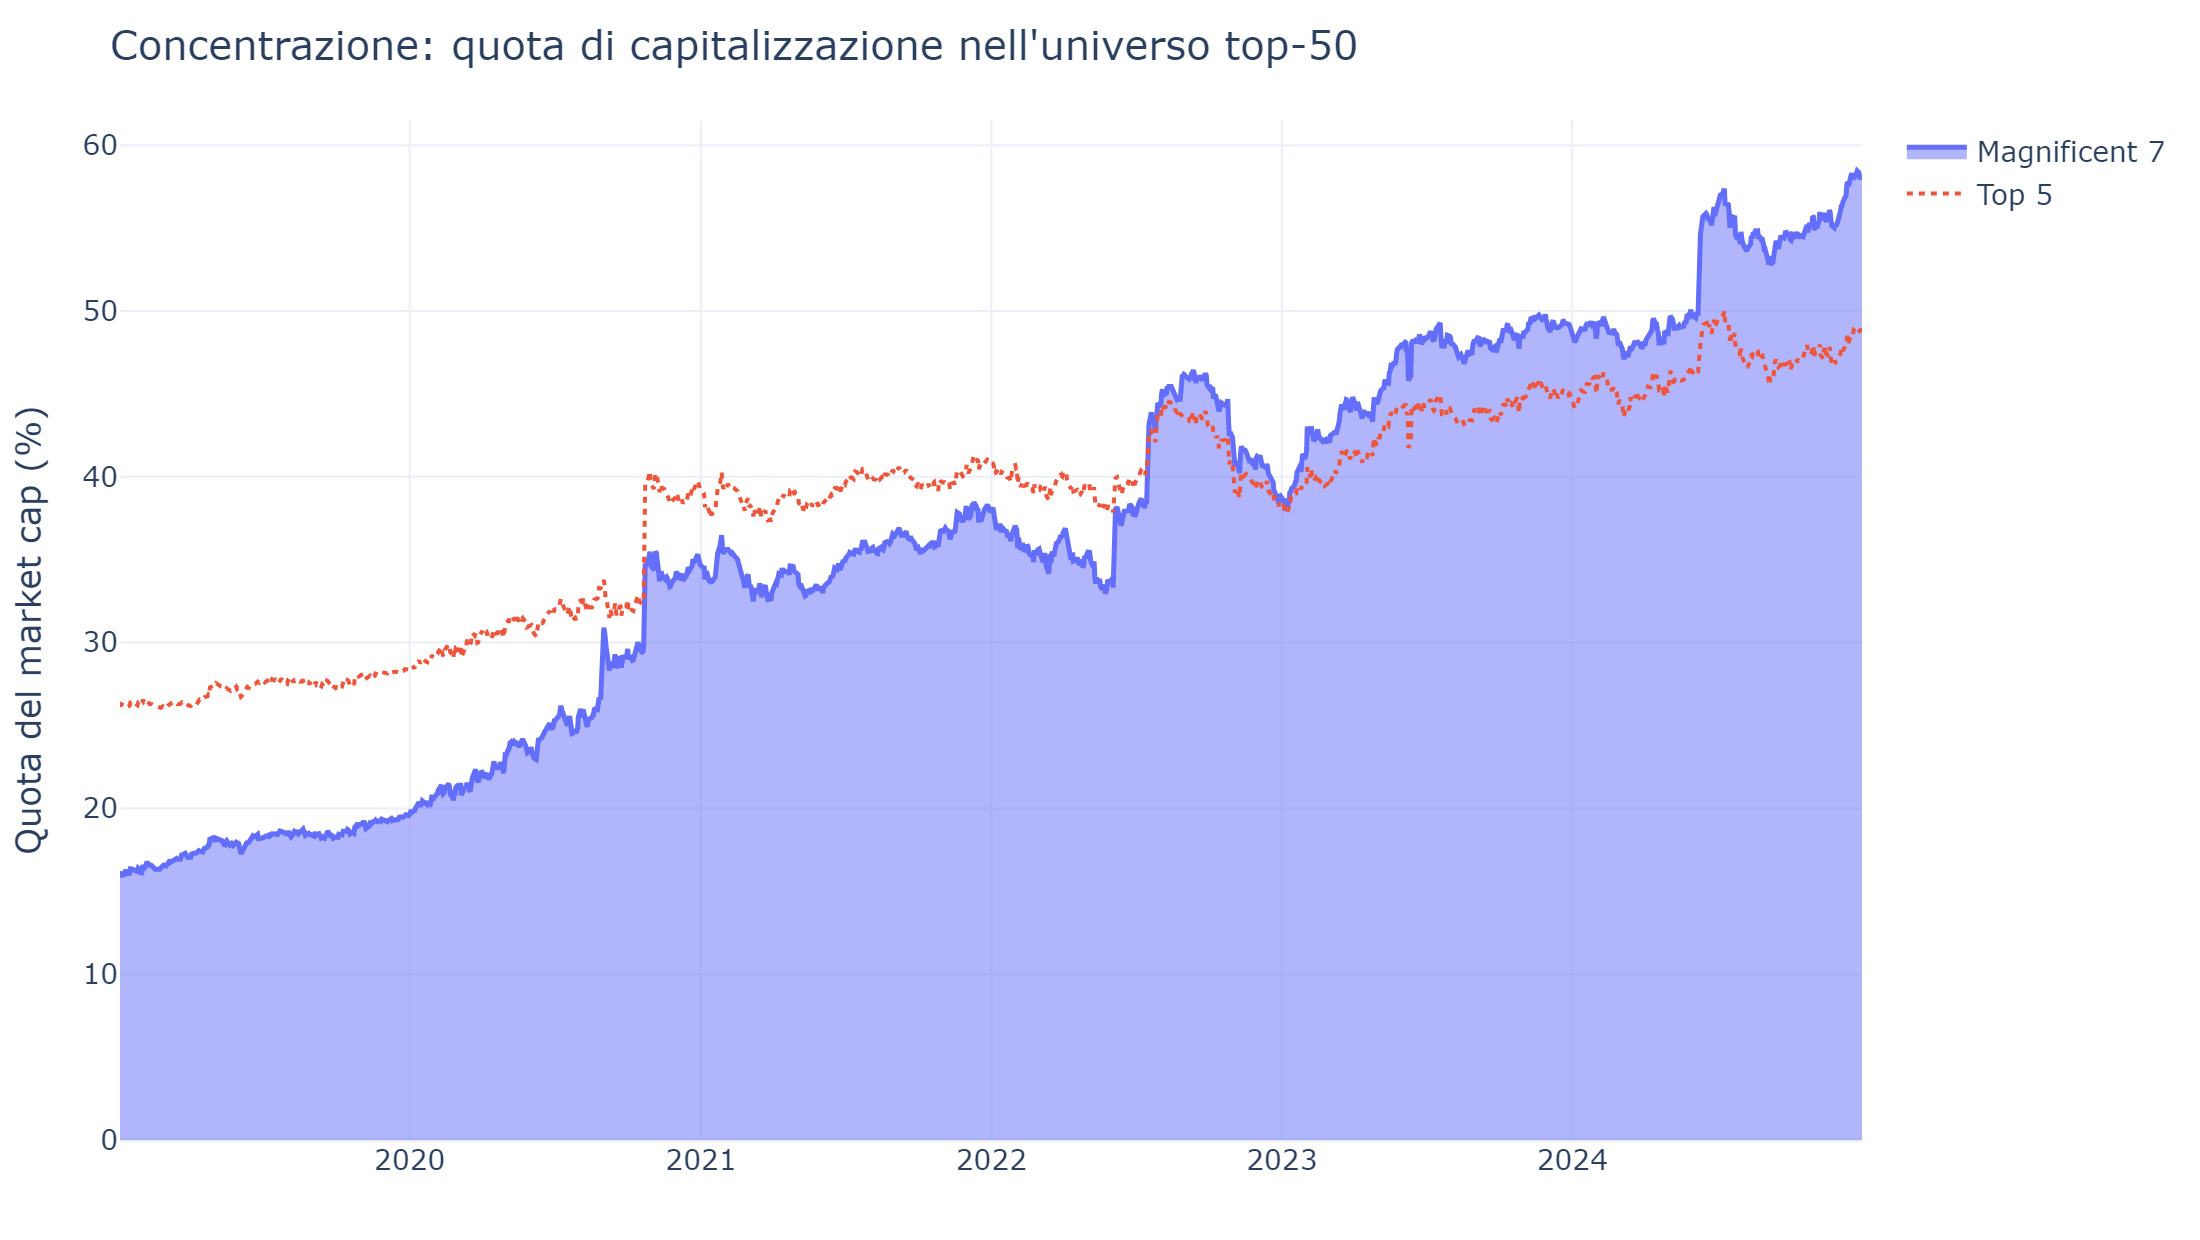
\includegraphics[width=\linewidth]{figures/concentration_chart.png}
  \caption{Concentrazione: quota combinata di capitalizzazione di mercato dei Magnifici Sette (e dei cinque maggiori titoli) all'interno dell'universo dei cinquanta maggiori costituenti, 2019--2024.}
  \label{fig:concentration}
\end{figure}

La Figura~\ref{fig:concentration} quantifica direttamente il trend di concentrazione. La quota combinata dei Magnifici Sette sulla capitalizzazione dei primi 50 titoli è salita da circa il $16\%$ all'inizio del 2019 a circa il $58\%$ alla fine del 2024 --- più che triplicata. Alla chiusura del periodo i soli cinque maggiori titoli rappresentavano quasi il $49\%$ dell'universo dei primi 50. Questo è il fatto strutturale che sottende ogni altro risultato dell'articolo.

\subsection{Struttura di correlazione}

\begin{figure}[H]
  \centering
  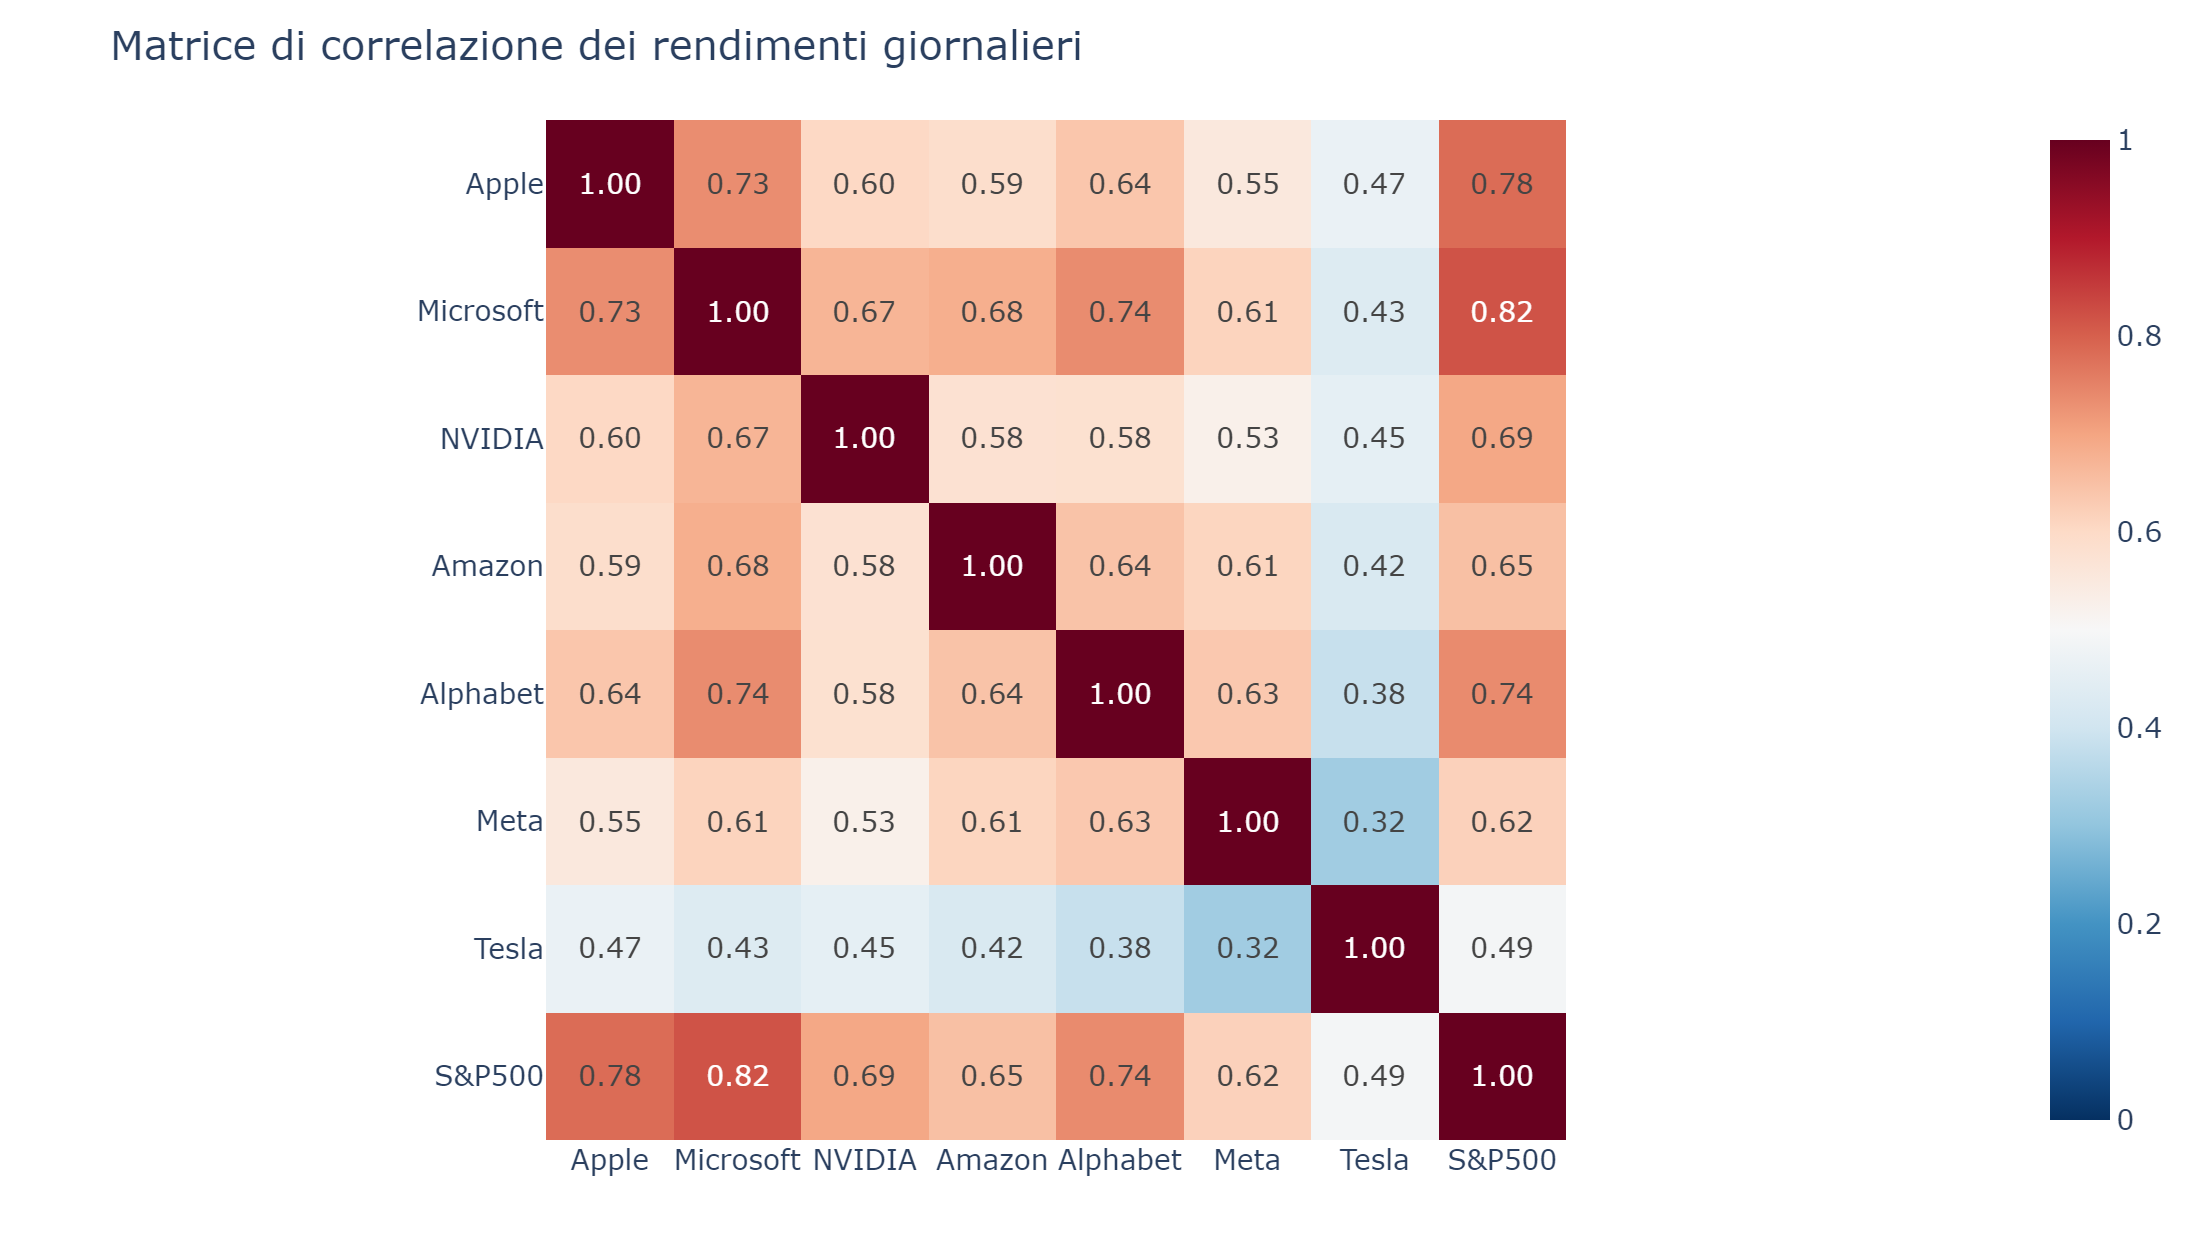
\includegraphics[width=0.8\linewidth]{figures/heatmap_chart.png}
  \caption{Matrice di correlazione di Pearson dei rendimenti giornalieri --- Magnifici Sette e S\&P500 (SPY), 2019--2024.}
  \label{fig:heatmap}
\end{figure}

La struttura di correlazione (Figura~\ref{fig:heatmap}) è rilevante per la questione della diversificazione. I Magnifici Sette esibiscono una correlazione media dei rendimenti giornalieri con l'indice di circa $0{,}68$; le correlazioni a coppie tra di loro scendono fino a circa $0{,}32$ (Tesla è la più idiosincratica). Le elevate correlazioni individuali con il benchmark si rinforzano meccanicamente man mano che queste aziende arrivano a dominare l'indice con cui sono correlate: un investitore che detiene l'indice detiene sempre più una scommessa tecnologica concentrata e mutuamente correlata, anziché un portafoglio diversificato.

\subsection{Performance corretta per il rischio}

Lo Sharpe ratio mobile a 12 mesi (Figura~\ref{fig:sharpe}) mostra che il vantaggio corretto per il rischio dell'indice ponderato per capitalizzazione rispetto alla versione equiponderata non è costante: i due indici si muovono insieme per gran parte del campione, con SPY che si stacca decisamente durante il rally guidato dall'IA del 2023--2024. Vi sono intervalli --- in particolare lo shock dei tassi del 2022 --- in cui l'indice equiponderato ha tenuto in modo paragonabile o migliore, a ricordare che la concentrazione è un'arma a doppio taglio.

\begin{figure}[H]
  \centering
  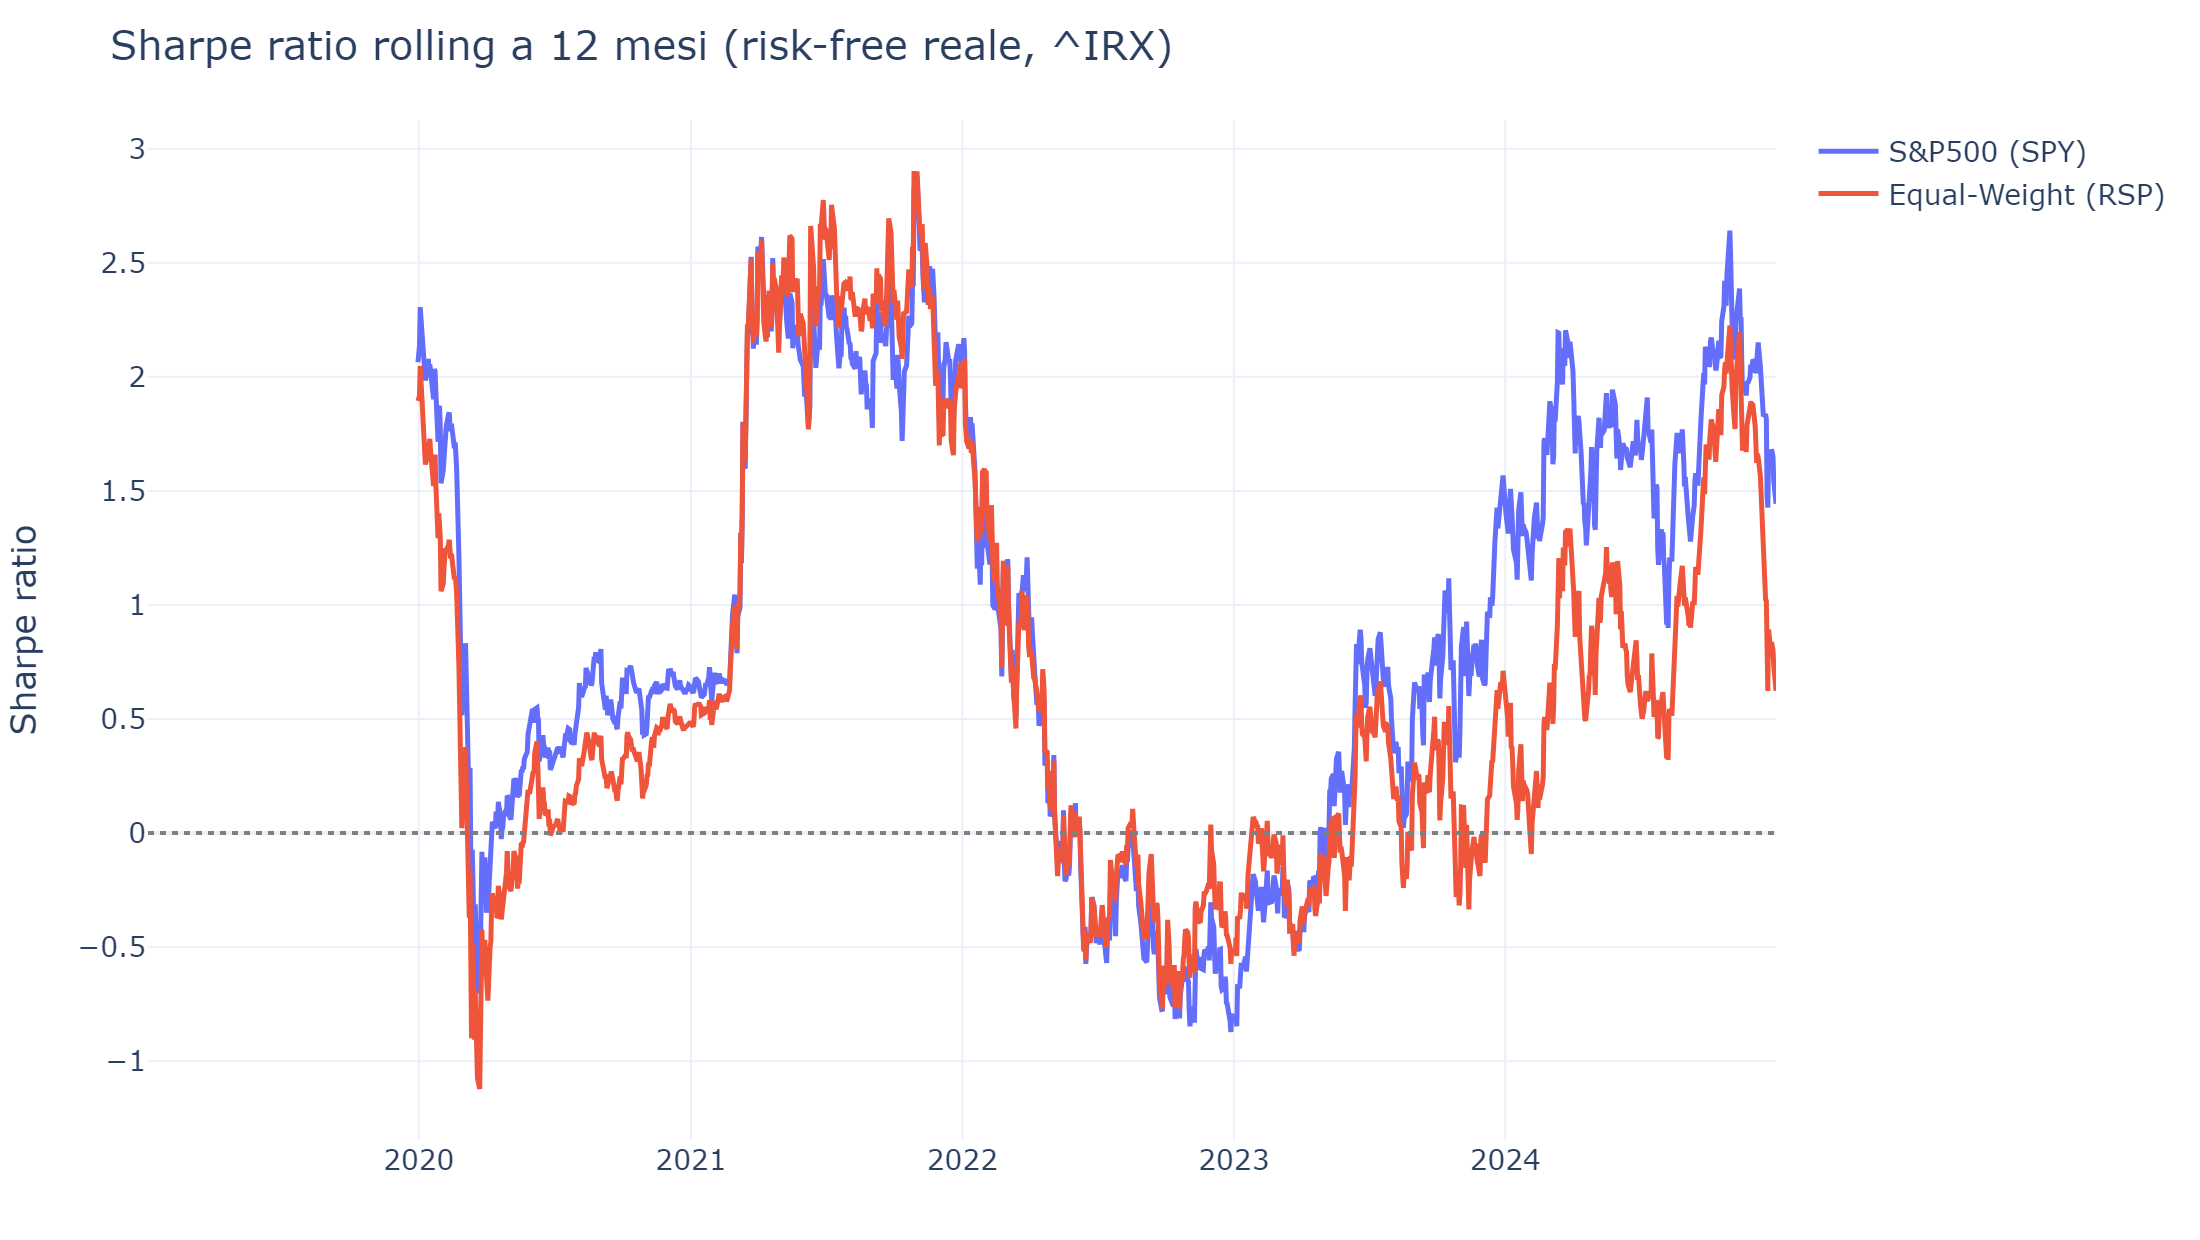
\includegraphics[width=\linewidth]{figures/sharpe_chart.png}
  \caption{Sharpe ratio mobile a dodici mesi: ponderato per capitalizzazione (SPY) rispetto a equiponderato (RSP), utilizzando il tasso privo di rischio realizzato.}
  \label{fig:sharpe}
\end{figure}

\subsection{Significatività statistica}

Il divario cumulato di $46$ punti percentuali tra l'indice ponderato per capitalizzazione e quello equiponderato è economicamente ampio, ma è statisticamente distinguibile dal rumore? Verifichiamo l'ipotesi nulla che la differenza media dei rendimenti giornalieri $d_t = r_t^{\text{SPY}} - r_t^{\text{RSP}}$ sia pari a zero, mediante un test $t$ per dati appaiati sulle $1{,}509$ osservazioni giornaliere. La differenza media corrisponde a circa $+3{,}0$ punti percentuali di sovra-rendimento annualizzato a favore dell'indice ponderato per capitalizzazione, ma con $t = 1{,}08$ e $p = 0{,}28$ \emph{non} possiamo rifiutare l'ipotesi nulla ai livelli convenzionali.

Questo apparente paradosso è istruttivo. Un vantaggio giornaliero piccolo rispetto alla volatilità giornaliera --- e perciò statisticamente non significativo ad alta frequenza --- può comporsi in una divergenza cumulata molto ampia nell'arco di sei anni. La sovraperformance complessiva è reale ed economicamente rilevante, eppure non costituisce prova statistica di un premio al rendimento persistente e sfruttabile; è coerente con l'idea che la concentrazione amplifichi un segnale giornaliero essenzialmente rumoroso. (Si noti che i rendimenti giornalieri presentano una lieve autocorrelazione, sicché il test $t$ sovrastima leggermente la dimensione effettiva del campione; la conclusione di non significatività è, semmai, conservativa.)

\section{Discussione}

\subsection{Implicazioni per l'EMH}

I risultati ammettono due letture. Secondo un'interpretazione rigorosa dei mercati efficienti, il dominio dei Magnifici Sette non è affatto un'anomalia: i loro prezzi riflettono semplicemente fondamentali eccezionali e correttamente anticipati (cloud computing, scala pubblicitaria e ciclo del capitale legato all'IA). Il fatto che un insieme noto e nominato di titoli abbia trainato gran parte del rendimento dell'indice non costituisce, di per sé, prova di inefficienza --- la forma semi-forte predice soltanto che non si possano ottenere rendimenti \emph{anomali} a partire da informazioni \emph{pubbliche}, e la concentrazione è stata di pubblico dominio per tutto il periodo. La lettura comportamentale, sulla scia di \citet{shiller1981} e \citet{debondt1985}, additerebbe invece la rapidità e l'ampiezza della rivalutazione del 2023--2024 come coerenti con un'iper-reazione e un momentum guidato dalla narrativa. I nostri dati non possono dirimere la questione; il problema della doppia ipotesi \citep{fama1991} implica che ogni verdetto dipende dal modello di pricing assunto.

\subsection{Il rischio di concentrazione per gli investitori passivi}

Merita enfasi un meccanismo che si auto-rinforza. L'investimento passivo ponderato per capitalizzazione acquista meccanicamente una quota maggiore di un titolo man mano che esso sale: man mano che le mega-cap crescono, i fondi indicizzati vi allocano quote sempre più grandi, il che sostiene la domanda e ne gonfia ulteriormente il peso. La diversificazione, principale argomento di vendita dell'investimento indicizzato \citep{markowitz1952}, viene così erosa silenziosamente dall'interno. Il divario di $46$ punti percentuali tra SPY e RSP è il prezzo di tale erosione quando la concentrazione ripaga; il drawdown più profondo del paniere Mag7 ($-43\%$) ne è il costo quando non ripaga.

\subsection{Cautele e interpretazioni alternative}

Tre cautele temperano le conclusioni. In primo luogo, i ``Magnifici Sette'' sono un costrutto col senno di poi: definire il gruppo come l'insieme delle aziende che \emph{hanno} vinto garantisce che escluderle deprima i rendimenti (un effetto di selezione/sopravvivenza). In secondo luogo, la finestra 2019--2024 è insolitamente favorevole a queste aziende; una finestra diversa produrrebbe un'entità diversa. In terzo luogo, le valutazioni elevate potrebbero essere pienamente giustificate dai fondamentali, nel qual caso non vi è alcuna ``bolla'' da sgonfiare né alcuna inefficienza da sfruttare.

\section{Conclusione}

Utilizzando pesi ricostruiti storicamente, un autentico benchmark equiponderato e il tasso privo di rischio realizzato, troviamo che la performance dell'S\&P500 nel 2019--2024 è stata in misura sostanziale un fenomeno dei Magnifici Sette: queste sette aziende sono cresciute dal $16\%$ al $58\%$ della capitalizzazione dei maggiori costituenti e spiegano circa il $35\%$ dei rendimenti cumulati dell'indice, con l'indice ponderato per capitalizzazione che supera il proprio gemello equiponderato di $46$ punti percentuali. La concentrazione è meglio intesa non come un'anomalia transitoria, bensì come una caratteristica strutturale dell'indicizzazione moderna ponderata per capitalizzazione --- una caratteristica che amplifica tanto i rendimenti quanto i rischi, e che complica la semplice equazione tra possesso dell'indice e diversificazione. Se ciò rappresenti un pricing efficiente di fondamentali eccezionali oppure un eccesso guidato dalla narrativa rimane, in coerenza con il problema della doppia ipotesi, formalmente indecidibile a partire dai soli rendimenti.

\bibliographystyle{plainnat}
\bibliography{references}

\end{document}
